\chapter{Methods} \label{sec:Methods}
The objective of the following sections is to outline the approach used to evaluate the feasibility of the model and then to improve its performance by means of model selection, data processing and applications specific design choices.

To evaluate the feasibility of this forecasting task the model can be divided into its' primary components so they could be developed and examined independently.

Since the inputs to the system can be divided into four  main components: sewage, cold-water, district heating usage and runoff from rainfall, so can the task of forecasting be split into these components. 

\textbf{The district heating} in Iceland is powered by geothermal heated water which is usually not circulated but rather exists the system (Note: some parts of the system might have have a closed loop system but in general it is pretty safe to assume that a substantial portion of the district heating water enters the sewer system. In order for a model to estimate this portion of the input, the most important variable is the ambient temperature. Variables such as wind speed and moisture may also have some effect but it is minuscule in relation to the temperature. Because the flow of district heating water changes quite slowly in relation to ambient temperature and because ambient temperature follows a daily pattern due to sunlight, it's better to use a 24 hour rolling average of the temperature as an input variable. See figure \ref{fig:DistrictHeatingRelationship} showing a simple linear relationship. In order to forecast this input a model only needs a temperature forecast which can then be turned into a forecast of the 24 hour rolling average by including prior forecast or observation values.

\begin{figure}[H]
\centering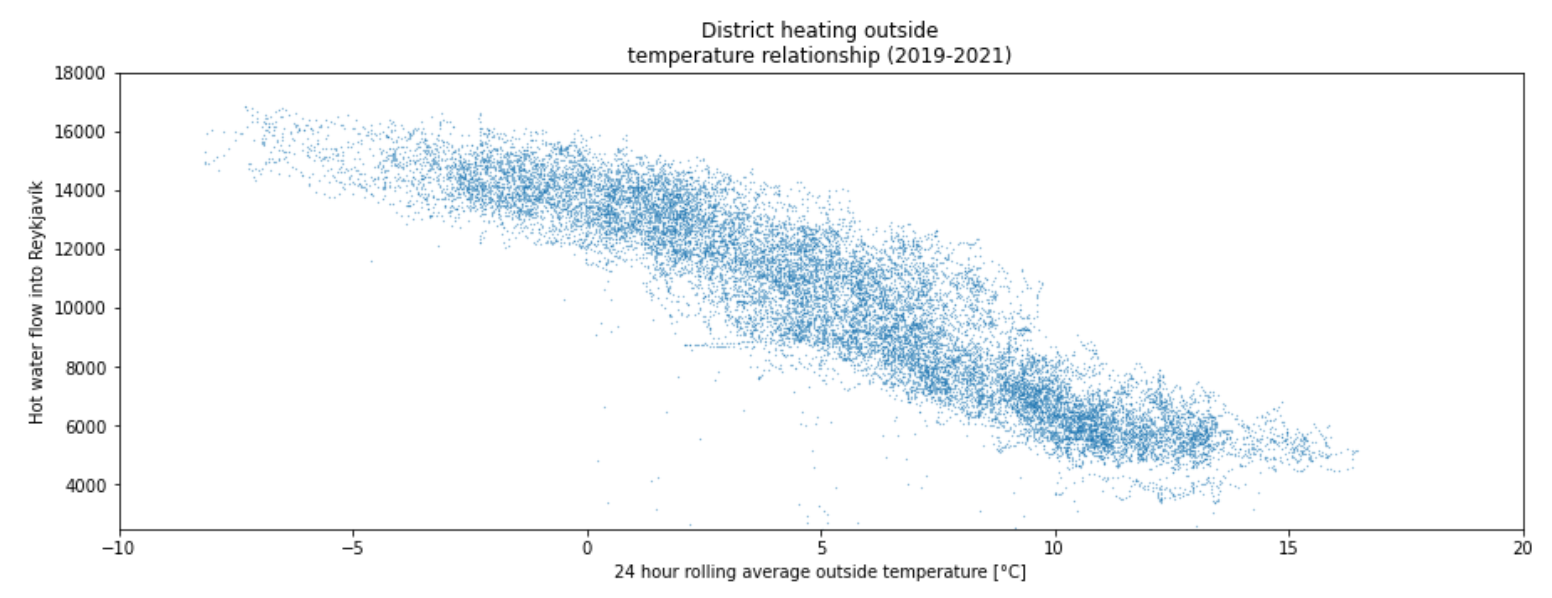
\includegraphics[width=\textwidth]{Pictures/Plots/DistrictHeatingTemperature.png}
\caption{Flow of hot water into Reykjavík and the 24 hour rolling average of the temperature in one location close to the center of Reykjavík. This demonstrates  the simple relationship between the two variables}
\label{fig:DistrictHeatingRelationship}
\end{figure}

\textbf{Cold-water usage and sewage} in residential neighbourhoods and most industrial neighbourhoods are not dependant on environmental variables but instead follow a very predictable daily and weekly pattern. Looking at examples of cold-water usage in a residential neighbourhood will show this. See figure \ref{fig:coldwaterusage} below. In order to forecast this input into the system it's only necessary to include the time of day and the day of the week as one-hot-encoded variables. One problem with this approach is that it assumes that the usage pattern remains constant over the whole period, which is not exactly the case. There may be other factors at play such as a growing population, holidays or other events which can alter this quantity but for sake of simplification this assumption will be used throughout the project. 

\begin{figure}[H]
\centering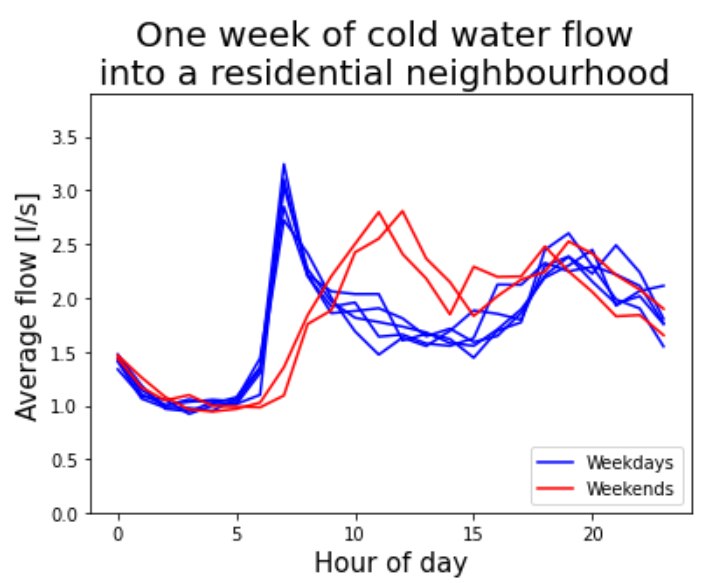
\includegraphics[width=0.5\textwidth]{Pictures/Plots/cold water usage.png}
\caption{Cold water usage in residential neighbourhood}
\label{fig:coldwaterusage}
\end{figure}

\textbf{Rainfall-runoff }is the last piece of the puzzle and is also the hardest of the three to model. The difficulty lies in two main factors:
\begin{itemize}
\item It's hard to get good\textbf{ observations} of all the rainfall over a given catchment.
\item The whole system is \textbf{highly non-linear and dynamic}. This includes the effect of antecedent precipitation, soil saturation, imperviousness of the surface and much much more.
\item The spatial distribution of rainfall can greatly affect the runoff. If a rainfall event is sufficiently concentrated in a small area a difference of just a few hundred meters can mean a difference of little-to-no increased runoff or surpassing the maximum capacity of a pumping station. (TODO: WRITE A BIT MORE ABOUT THIS IN THE LITERATURE REVIEW)
\end{itemize}

Because of the effect of antecedent precipitation the model will not only need to get the most recent observations but also observations for some time prior to the current observation. This may be included as the observations themselves or a predefined weighted sum of previous observations for simplification.

A problem arises with the need for forecasting rainfall partly because of the importance of spatial information. While the district heating only requires a rolling temperature from a single point within the region of interest, such is not the case for rainfall. The two options discussed in the literature review (TODO: WRITE MORE ABOUT THIS IN THE LITERATURE REVIEW), numerical weather predictions (NWP) and radar nowcasts have different pros and cons. Because a radar nowcast was not available for this project it will not be examined further for forecasting purposes. However experiment 1 compares rain-gauge observations to radar observations for flow simulations. (MAYBE THIS NEEDS TO BE ELABORATED ON) Thus for the forecasting model in experiment 2, numerical weather prediction data is used to forecast rainfall. 

One major problem with using numerical weather predictions to predict drainage flow is that another data source may be needed to include information about antecedent wetness. This may be included with the use of rain-gauge observations for the first step but since rain-gauge observations can't be known in advance it's hard to include this information at, for example, the 24 hour forecast since then a full day is missing observations from a rain-gauge. 

The precipitation forecast used in this study is the one made by the Icelandic Meteorological Office, which has used the HARMONIE - numerical weather prediction model since 2011 \cite{vedurstofaharmonie}. This forecast has a 2x2km spatial resoltuion a 1-hour temporal resolution and a 66-hour forecast horizon.

It's important to note several things about each of the data sources in order to understand the approaches used to quantify the uncertainty of each model. 

While the radar data is technically a direct observation, it cannot be treated as a ground truth  of rainfall observations. There are several reasons why this is the case but the main one being that the relationship between what is actually being observed, the radar echo, and actual rainfall is not fixed. To estimate rainfall from radar echo the convention is to use the so-called Z-R relationship $Z=AR^b$ which is governed by the distribution of raindrop size within a given storm at a given time, which can vary greatly\cite{ZRrelationship}.  Because of the uncertain nature of this relationship the rainfall distribution given by radar observation must be treated as an estimate with a given error by itself.

Therefore the radar data can not be used to evaluate the performance of the NWP model by acting as a ground truth. The Radar data can however be used in the evaluation of the precipitation nowcasting model, since the objective of that model is not to forecast rainfall but radar echo. 

To estimate the uncertainty of radar estimated rainfall and NWP forecasts rain-gauge data will be used, since they offer the only direct observation of rainfall available. The main drawback of this approach however is that rain-gauge observation are only observations of rainfall at a given point while NWP and radar based rainfall-estimates estimate rainfall over a given area. 


\subsection{Rain-gauge data}
The rain-gauge data time series used in the following experiments includes data from the start of 2015 to the end of 2020 collected and supplied by the Icelandic Meteorological Office. The rain-gauge in question is located right next to the Icelandic Metiorilogical Office and was thought to be the most reliable available rain-gauge for this project. The data was originally from a time series of 10-minute interval observations of the height of the rain-gauge collector. The data is then aggregated to hourly values and reviewed manually by staff at IMO. The only further processing applied to the data is a differencing operation to compute the change in water level over the duration of the hour and then all negative values are replaced with 0. The biggest negative values appear at the moments where the collector is emptied but can also include small negative values caused by evaporation from the collector. 

% Not sure what this manual review involves precisely, but it might be good to get some more details. 
% \begin{table}[H]
% \centering
% \caption{Rain gauges}
% \label{tab:raingaugetable}
% \begin{tabular}{@{}lSSSSS@{}}
% \toprule

% % Some other variables to consider : Station id, name of station, GPS location of the station, frequency of measurements (10 min for most or all rain-guages intially and then hourly in the manually reviewed dataset. 
% {id} & {name} & {GPS} & {frequency} & {start date} & {manual review} \\ \midrule
% 1473  & { Straumsvík }              & { 64°02' , 22°02' } & ? & { 2005-08-22 } & {yes} \\ 
% 1474  & { Garðabær - Urriðaholt }   & { 64°04' , 21°54' } & ? & { 2019-02-11 } & {yes} \\ 
% 1475  & { Reykjavík }               & { 64°07' , 21°54' } & ? & { 2005-08-22 } & {yes} \\ 
% 1478  & { Reykjavík Geirsnef }      & { 64°07' , 21°50' } & ? & { 2020-02-11 } & {yes} \\ 
% 1481  & { Hólmsheiði }              & { 64°06' , 21°41' } & ? & { 2008-01-11 } & {yes} \\ 
% 1482  & { Reykjavík Víðidalur }     & { 64°06' , 21°47' } & ? & { 2019-01-16 } & {no}  \\ 
% 1485  & { Bláfjöll úrkomustöð }     & { 63°58' , 21°39'} & ? & { 2005-08-22 } & {yes} \\ 
% 1578  & {Skrauthólar}               & ? & ? & { 2020-05-13 } & {no}  \\  

% 1490  & {Grindavík}                 & ? & ? & { 2005-08-22 } & {no} \\ 
% 1868  & {fíflholt}                  & ? & ? & { 2005-08-22 } & {no} \\ 
% 1490  & {Hellisskarð}               & ? & ? & { 2005-08-22 } & {no} \\ 
% 1779  & {Hvanneyri}                 & ? & ? & { 2005-08-22 } & {no} \\ \bottomrule
% \end{tabular}
% \end{table}

\subsection{Drainage data}
% The Reykjavík drainage system is roughly split into two main subsystems, one is called Skerjafjarðarveita and the other Sundaveita. These roughly constitute the northern and southern parts of Reykjavík. Within each system are a number of pumping stations and each system has a wastewater treatment plant. 

The drainage dataset consists of hourly averages of the flow from two drainage flow sensors (See \ref{sec:Case study} for details about problems with this data). These sensors are located in seperate pumping stations known as Boðagrandi and Gelgjutangi. Gelgjutangi is noteable because it is the oldest pumping station still in use in Reykjavík and gets its wastewater from the area highlighted in [figure name and id]. This system is thought to collect a relatively high proportion of the rainfall-runoff within its catchment and was thus considered a good candidate.

[I might include a single diagram even that shows the locations of each of the two pumping stations in the table above with the ID of each station displayed as well as a rough sketch of the catchment for either station]



\subsection{Numerical weather prediction data}
The numerical weather prediction data used in these experiments was provided by the Icelandic Meteorological office. The data included only the variable for the cumulative precipitation at 0m above ground, or in other words, estimated rainfall. The forecast has a forecast horizon of 66 hours, temporal frequency of 1 hour and spatial resolution of 2x2km and is updated every 6 hours. 

The accuracy of this forecast can be evaluated in and of itself by comparing rain-gauge observations with estimated rainfall. (this is something to do later) That can then be compared with the accuracy of radar estimated rainfall. 




\section{Data Processing}
This section will cover the specific methods used and the reasoning behind their usage.


\subsection{Radar data processing}
For more information about the radar data and data sources see the section \ref{sec:Case study}. The primary objective of the radar data processing is to turn the raw radar data into a 2D distribution of rainfall over the area of interest. Initially the radar data in this particular data set is available as a sequence of 420 by 120 matrices of 8-bit unsigned integer values along with metadata where the key information includes: A description of the radar scanning strategy, values for scaling and offsetting to restore the original range of echo data from the 8-bit unsigned integer values, the value used to represent missing data, the timestamp of the scan and the location of the radar. The radar scanning strategy describes the orientation, angles and distances needed to project the values into their respective locations in 3D space around the radar. These include the range bins, to indicate the distance to the start and end of each independent volume, the azimuth angles, which describe the angle of rotation about the spin-axis of the radar where the 0$^{\circ}$  and 360$^{\circ}$ face north and 180$^{\circ}$ south, and lastly the width of the radar beam. The two most common radar strategies used during the six year period from which the data was gathered can be seen in figures \ref{fig:radarstrat1} and \ref{fig:radarstrat3}. 


\begin{figure}[H]
\centering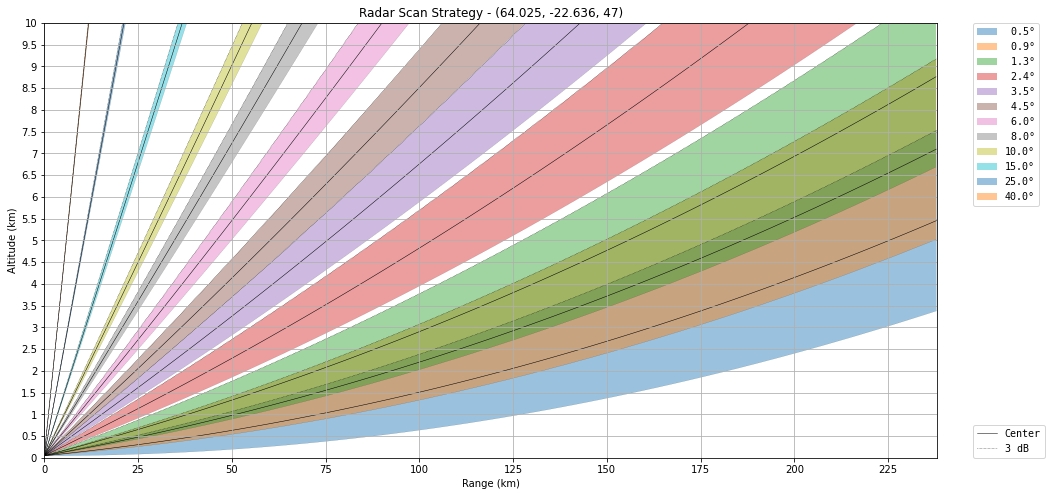
\includegraphics[width=\textwidth]{Pictures/Diagrams/Radar strategies/Strategy 1.png}
\caption{Radar strategy 1}
\label{fig:radarstrat1}
\end{figure}

\begin{figure}[H]
\centering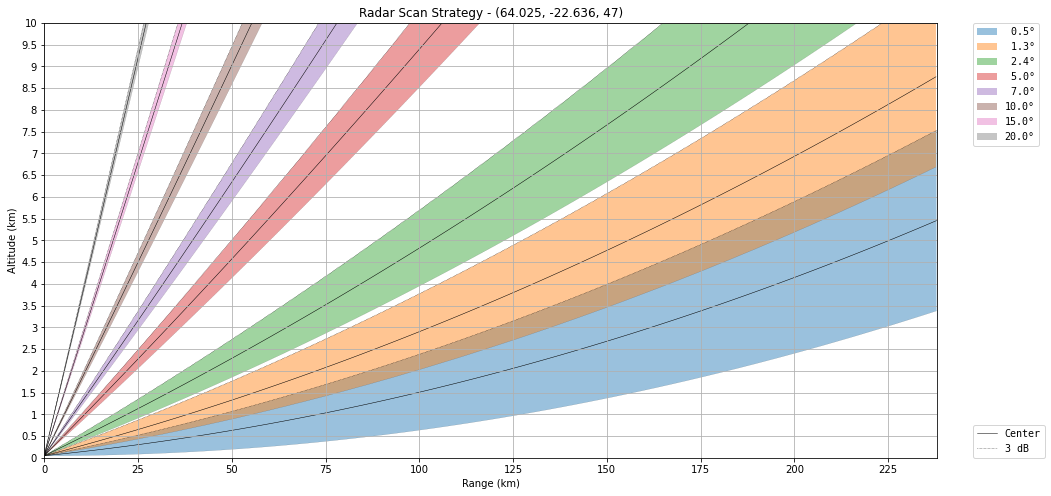
\includegraphics[width=\textwidth]{Pictures/Diagrams/Radar strategies/Strategy 3.png}
\caption{Radar strategy 2}
\label{fig:radarstrat3}
\end{figure}
Normally the data from different strategies can not be used directly with the same model since there might be different numbers of elevation angles and so more layers of radar data but also because the elevation angles might be be the same and so the layers wouldn't contain estimates of the same volume. To ensure the data can be used with a single model all radar data needs to include more or less the same volumes of space. This can be done by computing a  a Constant altitude plan position indicator (CAPPI). The CAPPI data is generated by calculating the corresponding position of each pixel in 3D space as well as deciding on a single elevation and pixel density and then interpolating the values at the desired points from the original data. This principle is demonstrated in figure \ref{fig:CappiPrinciple}. These projections have to take into consideration the curvature of the radar beam as it refracts in the atmosphere as well where the fixed elevation above sea level is compared to the surface below considering the curvature of the earth.The method used in this paper was a slight variation on CAPPI called pesudo-CAPPI, which fills areas above and below available radar beams with interpolation and will uses the lowest available layer even when the true radar beam is at much higher elevation. Usually, with CAPPI, these values would be left out. The implementation of the pseudo-CAPPI used in this paper came from the python library \textit{wradlib} \cite{hess-17-863-2013}.

\begin{figure}[H]
\centering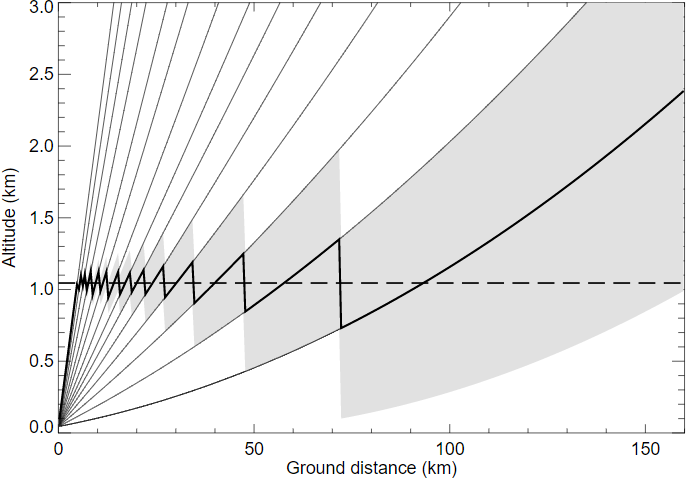
\includegraphics[width=\textwidth]{Pictures/Diagrams/CappiPrincipleCropped.png}
\caption{(\cite{CappiDemo}) Principle of CAPPI construction at 1 km above radar. The construction uses 14 elevation angles. The dashed line represents a presudo-CAPPI height of about 1km above the radar. The solid bold line represents the closest beam centers to the selected height at a given distance from the radar}
\label{fig:CappiPrinciple}
\end{figure}

Aside from just radar strategy another characteristic of the data changed between 2015 and 2020. When converting raw radar data into echo the following formula is used:  $dBZ = offset + gain * data$. 
By doing this the data can be stored in 8-bit unsigned integer format as values between 0 and 255. At around the start of 2018 the data started to be stored in a new data format. The old one being .h5 and the new one being .hdf5. For the data used in this project the offset for all files stored in the old data format .h5 had an offset of -30 and a gain of 0.4 while those stored in the newer format .hdf5 had an offset of -32 and a gain of 0.5. This was taken into consideration when the original reflectivity was computed for all the data.  

The pCAPPI reflectively images have a resolution of 600x600 pixels and are computed for a constant height of 2km. Since the maximum range of the radar data is about 240km or about the pixels derived from the data cover a roughly 800x800m area, although this does not represent the original resolution of the data since those volumes aren't equally spaced and the resolution drops with distance since the volume covered by the same radar beam grows about fourfold as the distance increases since the area grows fourfold while the range bins are equally spaced. The length of the range bins from the raw data are 2km and the difference in angle between adjacent radar beams is 6/7th of a degree since a full rotation of 360 degrees is 420 equally spaced azimuth angles. For the first 3 years and 3 months the data was recorded every 15 minutes after which the new radar strategy was adopted and the data was recorded every 5 minutes but with fewer elevation angles. The relative density of these values can be seen in figure \ref{fig:CappiResolution} along with the position of the weather radar. Marked on the figure are also the positions of the rain-gauges operated by the Icelandic Meteorological office within this area, some of which can be used for validation purposes of the radar Data.  

\begin{figure}[H]
\centering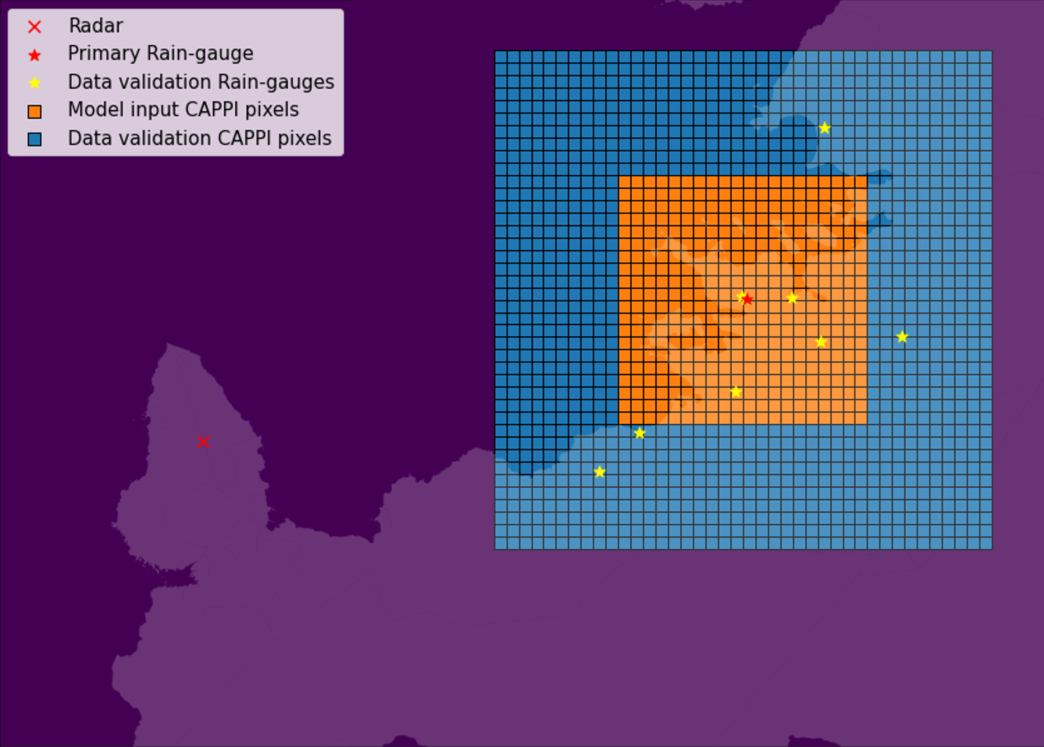
\includegraphics[width=\textwidth]{Pictures/Diagrams/CappiDataValidation.png}
\caption{Radar and primary rain-gauge positions and the pCAPPI pixels overlayed on a map including the Reykjanes peninsula and Faxaflói bay. The blue pixels represent the pCAPPI pixels specifically generated for the project and the orange pixels represent those used as input into the rainfall-runoff simulation models}
\label{fig:CappiResolution}
\end{figure}

The next step involves comparing the radar estimated rainfall with the rainfall observed by the rain-gauges. To convert the radar echo to rainfall estimates the equation is 

\section{Model}


\subsection{Drainage forecast from precipitation forecast}



\subsection{Precipitation forecasting models}
The first part of the complete model is the precipitation forecast itself. 



\subsection{Rainfall-runoff model}
The second part of the model is the rainfall-runoff model. The target variable for this model is the drainage flow at one or more pumping stations in the Reykjvaík drainage system. All parts of the drainage system in Reykjavík get input from one or more of the following sources: water used in for district heating, sewage and other wastewater, and rainfall-runoff. It should be highlighted that the district heating system in Iceland is not a closed loop and thus in most neighbourhoods will often enter the same route as rainfall water. That can be into the sewers or to a separate drainage system for non-sewage wastewater. 

If a model is supposed to forecast drainage flow it must have information about that predicts each of these sources. The first source, water for district heating use is relatively predictable in that mainly depends ambient outside temperature. The second source, sewage and other wastewater is relatively predictable in residential neighbourhoods, since they will follow very consistent patterns over the period of a day or a week. What remains to be predicted is the surface water from rainfall-runoff. 

% I think it's important to note here that getting the absolute best performance possible from this model wasn't the objective. The point of this subsection was a proof-of-concept for 1 or 2 kinds of models. The original thinking was that not too much focus would be put on this part because there was already going to be a lot of uncertainty in the feasibility of the overall model. 
The following experiment demonstrates the feasibility of modeling rainfall-runoff with the available data without incorporating future forecasting. The types of data sources considered in this experiment are: hourly average temperature data, raw 10 minute resolution rain-gauge data hourly and manually adjusted rain-gauge data. The target variables considered are hourly average flow measurements from several drainage stations. Before analysis and selection of variables, the entire year of 2020 was reserved for later testing purposes so as not to affect the decision process. 

To select the input and target variables several criteria were considered. Firstly, a dataset with an abundance of data was favored. All sensors with less than a year of data after 2020 had been removed were eliminated from consideration. For a visualization of the relative abundance of data was available for each target and input variable see figure \ref{fig:missingdata}.  Secondly, the wastewater treatment plants were eliminated as candidates since the size of these catchments means that spatial information becomes more important, which was not the objective of this demonstration. Thirdly the the system in question had to be a combined sewer to ensure that enough of an effect from rainfall-runoff could be observed for the demonstration. For this third factor, the correlation between the hourly accumulated rainfall and drainage flow was used as as a metric. To ensure that the the time-delay between maximal correlation of rainfall and drainage flow wouldn't affect the choice, the correlation between each rain-gauge-drainage flow meter pair was computed with up to 20 hours delay and the maximal correlation for each pair was used. The results of this can be seen in figure \ref{fig:maxcorrpairs}. 

\begin{figure}
\centering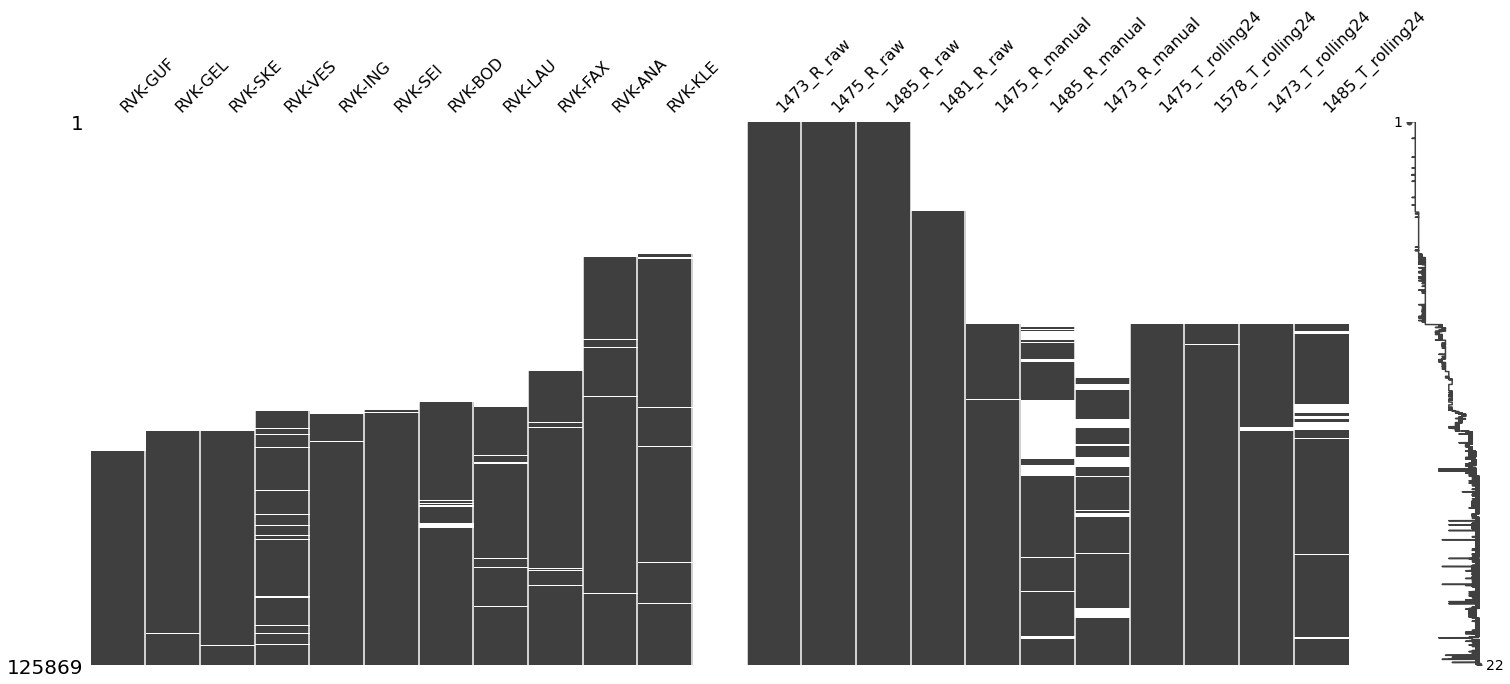
\includegraphics[width=\textwidth]{Pictures/Plots/missingdata.png}
\caption{Visualization of relative abundance of data for each of the target variables (left of the gap) and each of the input variables with data available since before 2019 (right of the gap)}
\label{fig:missingdata}
\end{figure}

\begin{figure}
\centering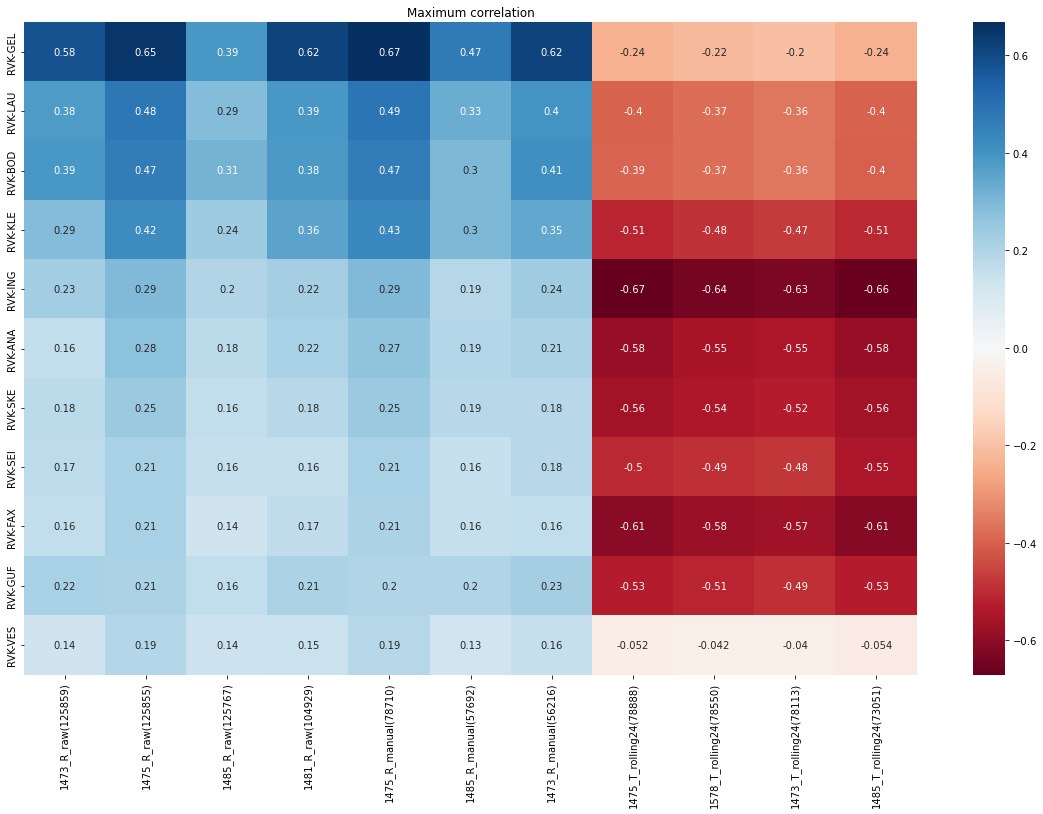
\includegraphics[width=\textwidth]{Pictures/Plots/max_corr_pairs.png}
\caption{Maximal correlation between hourly average drainage flow and hourly accumulated rainfall from each drainage flow sensor and rain-gauge not removed on the basis of a lack of data}
\label{fig:maxcorrpairs}
\end{figure}

For this experiment it was decided that two target variables be used: "RVK-GEL" and "RVK-BOD". The input variables selected were both the rain-gauge and temperature data from sensor 1475 partly due to their high correlation with both variables and partly since the rain-gauge data was available as both raw and manually corrected.

%It might be good to include some further information about these drainage systems. For example I think both have quite a large industrial neighbourhoods and one is also very close to and responsible for the drainage of a 2x4 lane highway intersection and is also one of the older, if not the oldest parts of the drainage system in Reykjavík. 

Several variations of models and input data were tested. The exact description of these variations is explained 

It must be taken into consideration that not that all rain water that falls onto the surface immediately enters the drainage system, let alone flows all the way to the drainage flow meter on the way out of the pumping station. To account for this lag, the simplest solution is to include previous rainfall observations in addition to the most recent. 
% NOTE: if the increased dimensionality isn't an issue, since there is an abundance of training and testing data, it might be interesting to check if using the raw 10-minute rain-gauge values instead of the aggregated hourly cumulative rainfall gives a better result. Different time-scales aren't an issue if you just include all the extra data-points as more variables rather than more observations. 
How many previous observations it makes sense to include will be different for each pumping station. A rule of thumb in urban hydrology is that water travels at about one meter every second so it might make sense to allow for at least the distance across the catchment from the pumping station but in reality it can take much longer for water to flow to the end of the system, since it will often be delayed on the surface, in soil, on buildings or other geological features, not to mention the fact that precipitation in the form of snow will undoubtedly have a much longer delay than rain. 

Because of the uncertainty of this choice it was decided compare the performance of a linear regression model using a differing amount of lagged variables. % I'm really not so sure about this approach and I don't trust the fact that the first experiments (which I have yet to conduct more thoroughly) show that the performance just continues to improve unto something like 2 weeks back, which is 336 variables, and that as without regularization. 

Although the performance of the model did continue to marginally improve as more and more delayed variables were added, most of the improvements were for observations less than 12 hours old and after about 48 hours the performance has more or less completely plateaued. 


\begin{figure}
\centering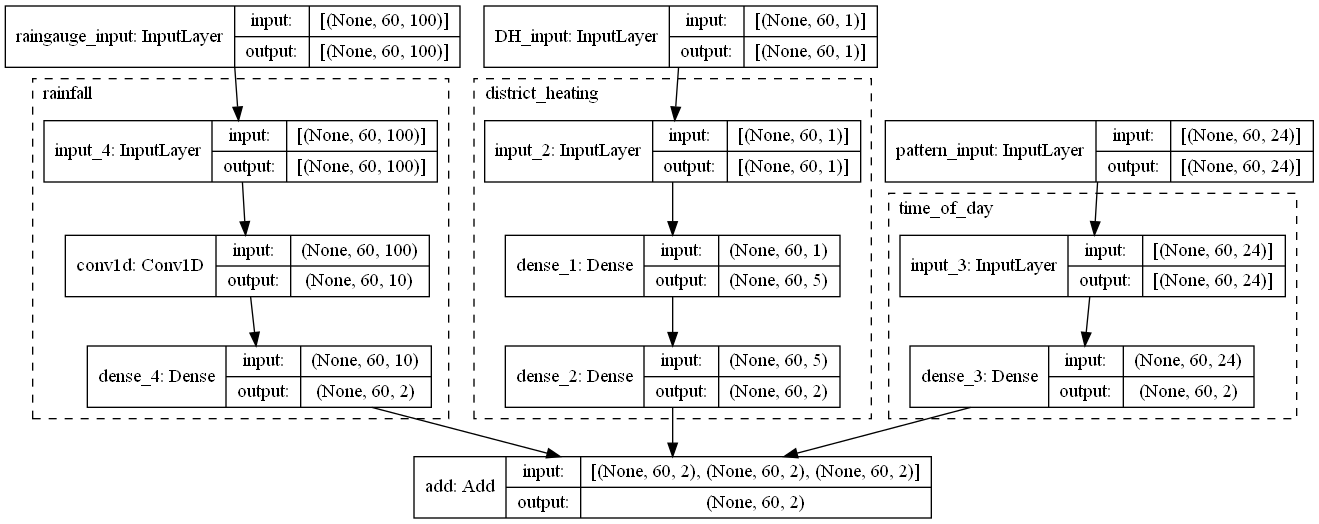
\includegraphics[width=\textwidth]{Pictures/Plots/conceptual.png}
\caption{Diagram of the conceptula model}
\label{fig:ConceptualModelDiagram}
\end{figure}



\section{Experiments}
\subsection{Choice of metrics}
The choice of the metric by which models are selected can greatly affect the final results. It's important to make a distinction between three different concepts:
\begin{itemize}
\item Objective function
\item Evaluation metric
\item Real world benefit
\end{itemize}
The objective function is picked for computational properties such as being differentiable with respect to the model's coefficients. The evaluation metric is used to select between models. The distinction between the latter two metrics is made because the real world benefit is often hard to calculate or measure and so the evaluation metric can be used as an approximation. Ideally all three are mutually optimal but this is often hard to achieve or prove. 

The main application drainage flow forecast considered in this project is early warning of potential overflow events. According to staff at the Veitur utility company in Reykjavík a warning at least 24 hours in advance is usually enough to prepare to make staffing and equipment preparations for such events. Since forecasts are updated every 6 hours the prediction distances used for evaluation will be those 24 to 30 hours into the future in order to include all observations of the target variable in the data set in the training and evaluation.

The models in this project are regression models but the task is one of classification. To convert the predictions into the desired binary classification form, a threshold is used such that if a model predicts the flow to be above the threshold, it's considered a positive prediction and otherwise a negative prediction. Binary classification models are usually evaluated based on the ratio of some combination of values from the confusion matrix shown in table\ref{table:ConfusionMatrix}

\begin{table}[htb]
\centering
\resizebox{0.4\textwidth}{!}{%
\def\arraystretch{1.5}%
\begin{tabular}{ccccl}
                                               &                         & \multicolumn{2}{c}{Predicted}                     & Total \\ \cline{3-4}
                                               & \multicolumn{1}{c|}{}   & \multicolumn{1}{c|}{p}  & \multicolumn{1}{c|}{n}  &       \\ \cline{2-4}
\multicolumn{1}{c|}{\multirow{2}{*}{Observed}} & \multicolumn{1}{c|}{p'} & \multicolumn{1}{c|}{TP} & \multicolumn{1}{c|}{FN} & P'    \\ \cline{2-4}
\multicolumn{1}{c|}{}                          & \multicolumn{1}{c|}{n'} & \multicolumn{1}{c|}{FP} & \multicolumn{1}{c|}{TN} & N'    \\ \cline{2-4}
\multicolumn{1}{l}{Total}                      & \multicolumn{1}{l}{}    & \multicolumn{1}{l}{P}   & \multicolumn{1}{l}{N}   & T    
\end{tabular}%
}
\caption{A confusion matrix for binary classification}
\label{table:ConfusionMatrix}
\end{table}

The simplest classification metric is accuracy, which is the ratio of correct prediction to total predictions. The number of true negatives is not a strong indicator of performance for this application due to its relative abundance and low importance in the data. The critical success index shown in equation \ref{eqn:CSS} is the accuracy when true negatives are removed from the equation.
\begin{equation}
\label{eqn:CSS}
CSS = \frac{TP}{TP + FN + FP}
\end{equation}This metric is still biased towards common events since they will have more chance occurrences of true positives. A modified CSS known as the Gilbert skill score (GSS) in equation \ref{eqn:GSS} takes into consideration the number of chance occurrences of true positives for a less biased score.
\begin{equation}
\label{eqn:GSS}
GSS = \frac{TP - TP_{random}}{TP + FN + FP - TP_{random}}
\end{equation}
Where
\begin{equation}
\label{eqn:TPrandom}
TP_{random} = \frac{(TP + FN)(TP + FP)}{T}
\end{equation}The last missing criteria for the evaluation metric is the threshold selected to represent a positive observation. The higher the threshold the more important the event but also the less common the event, thus making evaluation of the model performance harder. Additionally the threshold will be different for each station since both the normal operating flow-rate and the maximum capacity of each pumping station will be different. Thus the threshold flow-rate is picked as a number within the following constraints:
\begin{itemize}
\item It is greater than the flow during all historical dry-weather conditions
\item It is low enough that it occurs at least 20 times every year
\end{itemize}





\subsection{Evaluation methodology}
All the models were trained with a weighted mean squared error loss function. The weights were computed using the drainage flow such that if the drainage flow surpassed a given flow rate it was given the corresponding weight as described in [table reference]. [table reference] shows how large a proportion of the dataset is larger than each of the thresholds. 

	


\begin{table}[H]
\centering
\caption{Gelgjutangi thresholds and weights}
\label{tab:tableThresholdsGel}
\begin{tabular}{@{}SSSSS@{}}
\toprule
         &                       & \multicolumn{2}{c}{Weight schemes} &  \\ \cline{3-4}
{Flowrate} & {Proportion} & {1} & {2} &  \\ \cline{1-4}
>0        &             {?}         & 1               & 1               &  \\ 
>100      &             {?}         & 2               & 1               &  \\
>200      &             {?}         & 4               & 1               &  \\
>300      &             {?}         & 10              & 1               &  \\
>400      &             {?}         & 20              & 1               &  \\
>600      &             {?}         & 30              & 1               &  \\
>800      &             {?}         & 40              & 1               &  \\
>1000     &             {?}         & 60              & 1               &  \\ \cline{1-4} \bottomrule
\end{tabular}
\end{table}


\begin{table}[H]
\centering
\caption{Boðagrandi thresholds and weights}
\label{tab:tableThresholdsBod}
\begin{tabular}{@{}SSSSS@{}}
\toprule
         &                       & \multicolumn{2}{c}{Weight schemes} &  \\ \cline{3-4}
{Flowrate} & {Proportion} & {1} & {2} &  \\ \cline{1-4}
>0        &                       & 1               & 1               &  \\
>25      &                       & 2               & 1               &  \\
>50      &                       & 4               & 1               &  \\
>75      &                       & 10              & 1               &  \\
>100      &                       & 20              & 1               &  \\
>125      &                       & 30              & 1               &  \\
>150      &                       & 40              & 1               &  \\
>200     &                       & 60              & 1               &  \\ \cline{1-4} \bottomrule
\end{tabular}
\end{table}



\subsection{Rain-gauge to runoff experiment}
The first experiment uses prior rain-gauge observations to predict current drainage flow.
\subsection{Radar to runoff experiment}
\subsection{NWP to runoff experiment}



\section{Performance requirements of different drainage applications}
The main application considered the reduction combined sewer overflows (CSOs). To achieve this goal there are several approaches, most of which require building of additional infrastructure such as additional pumps, larger reservoir or other control mechanisms. For any solution that uses control mechanisms to reduce CSOs it is necessary to have some sort of input mechanisms 




\cite{ThorndahlRadar}